\section{Efficiency}\label{sec:efficiency}
Next to the correctness, the efficiency of the proposed method is the most important metric to determine its feasibility. % TODO: maybe a better wording?
The main question is if or from what table size the proposed method is faster than the naive method. This becomes even more interesting as each positive guess of the model has to be verified using the naive algorithm to increase the accuracy. % TODO: ref to model

The following experiments explore the efficiency of the proposed method in comparison to the naive algorithm and which parameters have the greatest influence on it. %! TODO: write better?


\subsection{Experiment Data}\label{subsec:efficiency-experiment_data}
The experiments in this section were conducted on a set of generated tables to control the size of the table as well as the number of unique and non"=unique columns. A small example of such a table can be seen in Table~\ref{table:efficiency-generated_table}. % chktex 18

The generated tables each have \num{10} columns and between \num{100} and \num{100000000} columns. To ensure the correct prediction by the model, the columns where generated in a specific way.
The unique columns are evenly incrementing for the first \num{50} rows, while the first two rows of the non"=unique columns contain the same value. The rest of each column contains distinct incrementing values which are mixed up to increase the time the sorting based naive algorithm takes to find unique columns. % TODO: ref to naive algorithm  % chktex 18

\begin{table}[!ht]
  {
    \centering
    \newcommand{\tablevdots}{\multicolumn{1}{c}{\vdots{}}}
    \setlength{\tabcolsep}{5pt}
    \caption[A table generated for the efficiency experiment]{A table generated for the efficiency experiment. The columns 0 and 1 do not contain any duplicates, the columns 2, 3 and 4 do. To guarantee that the model guesses the unique and non-unique columns correctly, the unique columns are evenly incrementing for the first 50 rows, while the duplicate value of the non-unique columns is in the first two rows.} % chktex 18
    \begin{tabular}{SSSSSS}
      \toprule
      {Index}       & {Column \num{0}} & {Column \num{1}} & {Column \num{2}} & {Column \num{3}} & {Column \num{4}} \\ \midrule
      0             & 0                & 0                & 100              & 100              & 100              \\
      1             & 1                & 1                & 100              & 100              & 100              \\
      2             & 2                & 2                & 93               & 93               & 93               \\
      3             & 3                & 3                & 45               & 45               & 45               \\
      % 4        & 4                & 4                & 16               & 16               & 16               \\
      % 5        & 5                & 5                & 87               & 87               & 87               \\
      % 6        & 6                & 6                & 32               & 32               & 32               \\
      \tablevdots{} & \tablevdots{}    & \tablevdots{}    & \tablevdots{}    & \tablevdots{}    & \tablevdots{}    \\
      % 46       & 46               & 46               & 2                & 2                & 2                \\
      % 47       & 47               & 47               & 73               & 73               & 73               \\
      48            & 48               & 48               & 89               & 89               & 89               \\
      49            & 49               & 49               & 39               & 39               & 39               \\
      50            & 91               & 91               & 60               & 60               & 60               \\
      51            & 77               & 77               & 49               & 49               & 49               \\
      % 52       & 54               & 54               & 23               & 23               & 23               \\
      % 53       & 70               & 70               & 30               & 30               & 30               \\
      \bottomrule
    \end{tabular}\label{table:efficiency-generated_table}

  }
\end{table}



\subsection{Base experiment}\label{subsec:efficiency-base_experiment}
The first experiment explores the efficiency of the proposed method compared to the naive algorithm. The generated tables that were used contained \num{3} unique and \num{7} non"=unique columns.  % chktex 18

Figure~\ref{fig:efficiency-base_experiment-plot} and Table~\ref{table:efficiency_csv-70percent} show that for tables with up to \num{100000} rows, the naive algorithm takes only a fraction of a second and is therefore faster than the proposed machine learning model. However, since the model takes a roughly constant time of half a second to compute its prediction, it becomes faster as the table size surpasses one million rows.

The column \enquote{Model: Validation} in Table~\ref{table:efficiency_csv-70percent} additionally illustrates that the validation time of the proposed method is proportional to the number of positive guesses by the model. This highlights the importance of a high accuracy as explained in Section~\ref{subsec:correctness_comparing-input-size}, because each false positive guess unnecessarily increases the time it takes to validate the guesses and therefore decreases the efficiency.

In conclusion, this experiment illustrates that for large tables loading the dataset and checking the columns for duplicates with the naive algorithm takes the most time. Ways to reduce the loading time will be explored in Section~\ref{subsec:efficiency-shorter_loading_times}. While a more efficient naive algorithm is not part of this thesis, Section~\ref{subsec:correctness_comparing-input-size} and~\ref{subsec:correctness_examine-false-guesses} deal with the question of how to decrease the number of false positive guesses.

\begin{figure}[ht]
  \caption[Compare the efficiency the proposed method and the naive algorithm]{This plot shows the total runtime of the naive algorithm and the proposed method to compute the unique columns as can be seen in Table~\ref{table:efficiency_csv-70percent}. The tables were saved in a CSV format.} % TODO: better caption
  \label{fig:efficiency-base_experiment-plot} % chktex 24
  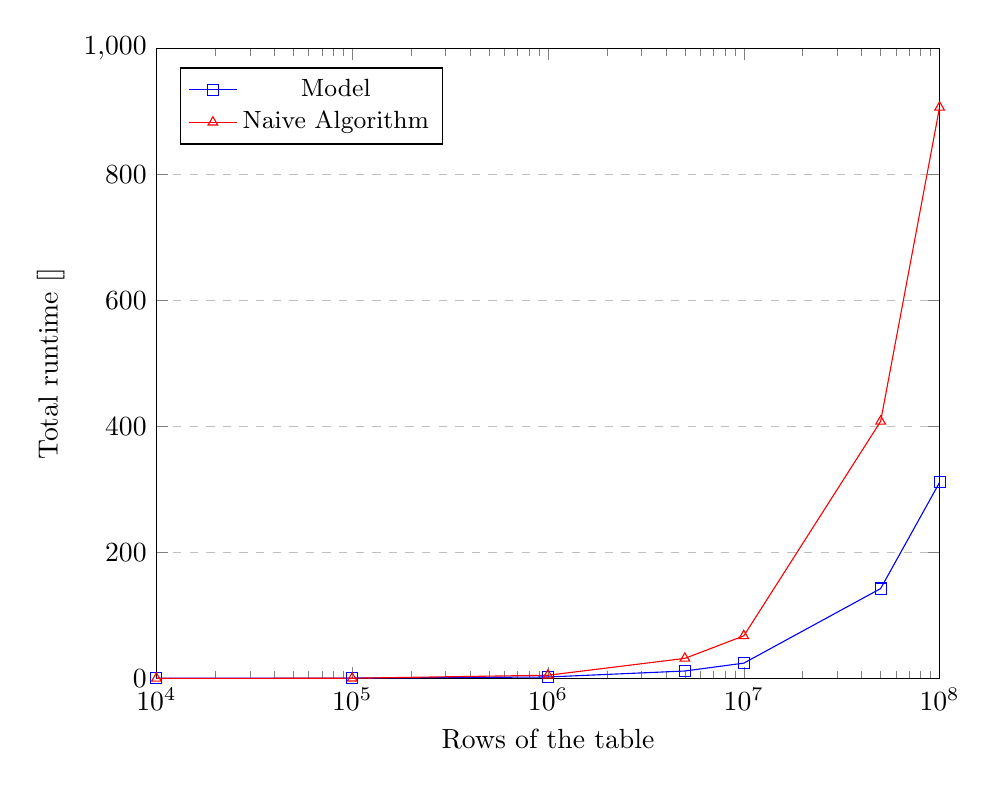
\begin{tikzpicture}
    \begin{axis}[
        % title={},
        xlabel={Rows of the table},
        ylabel={Total runtime [\si{\second}]},
        xmin=10000, xmax=100000000, xmode=log,
        ymin=0, ymax=1000,
        % xtick={0,1000,100000,10000000,100000000},
        % ytick={0,20,40,60,80,100,120},
        legend pos=north west,
        ymajorgrids=true,
        grid style=dashed,
        scale only axis,
        width={\linewidth-62pt},
        height=8cm
      ]

      \addplot[
        color=blue,
        mark=square,
      ]
      coordinates {
          (100.0,1.0835406184196472) (1000.0,0.4514627978205681) (10000.0,0.4591604061424732) (100000.0,0.5741918832063675) (1000000.0,2.2600879333913326) (5000000.0,11.771335251629353) (10000000.0,24.25790297240019) (50000000.0,142.64984269440174) (100000000.0,311.1732710637152)
        };
      \addplot[
        color=red,
        mark=triangle,
      ]
      coordinates{
          (100.0,0.0039823874831199) (1000.0,0.0037141181528568) (10000.0,0.0264939442276954) (100000.0,0.3022922314703464) (1000000.0,5.0495885498821735) (5000000.0,31.796920645982027) (10000000.0,67.54112743958831) (50000000.0,408.1332451477647) (100000000.0,906.6464131213723)
        };
      \legend{\small Model, \small Naive Algorithm}

    \end{axis}
  \end{tikzpicture}
\end{figure}


\begin{table}[htb]
    \centering
    \begin{tabular}{@{}cccccccccc@{}}
        \toprule
        Rows & Columns & ML: Loading & ML: Compute Time & ML: Loading & ML: Validation Time & ML: Total & Naive: Loading & Naive: Compute Time & Naive: Total \\
        \midrule
        100 & 10 & 0.0013715997338294 & 1.081736620515585 & 0.0013715997338294 & 0.0001396164298057 & 1.0835406184196472 & 0.0035197585821151 & 0.0004606023430824 & 0.0039823874831199 \\
        1000 & 10 & 0.0017428211867809 & 0.448739793151617 & 0.0017428211867809 & 0.0006883814930915 & 0.4514627978205681 & 0.0017647370696067 & 0.001948557794094 & 0.0037141181528568 \\
        10000 & 10 & 0.0060491673648357 & 0.4461151845753193 & 0.0060491673648357 & 0.0066703855991363 & 0.4591604061424732 & 0.0049485117197036 & 0.021544512361288 & 0.0264939442276954 \\
        100000 & 10 & 0.0453519634902477 & 0.4520450010895729 & 0.0453519634902477 & 0.0762417986989021 & 0.5741918832063675 & 0.0453673861920833 & 0.2569229155778885 & 0.3022922314703464 \\
        1000000 & 10 & 0.4341592788696289 & 0.4540174268186092 & 0.4341592788696289 & 1.3692879006266594 & 2.2600879333913326 & 0.4268940836191177 & 4.622690767049789 & 5.0495885498821735 \\
        10000000 & 10 & 4.655362159013748 & 0.4464701749384403 & 4.655362159013748 & 19.115534022450447 & 24.25790297240019 & 4.606263380497694 & 62.93486054614186 & 67.54112743958831 \\
        100000000 & 10 & 52.42867323383689 & 0.4439504966139793 & 52.42867323383689 & 257.90396685898304 & 311.1732710637152 & 52.22971136868 & 854.4166974648833 & 906.6464131213723 \\
        5000000 & 10 & 2.4758735559880733 & 0.4505492337048054 & 2.4758735559880733 & 8.824372578412294 & 11.771335251629353 & 2.4555414877831936 & 29.34137427061796 & 31.796920645982027 \\
        50000000 & 10 & 27.298193652182817 & 0.4581984207034111 & 27.298193652182817 & 114.69358796998858 & 142.64984269440174 & 27.074549317359924 & 381.0586917251349 & 408.1332451477647 \\
        \bottomrule
    \end{tabular}
\end{table}


\subsection{Reduce loading times}\label{subsec:efficiency-shorter_loading_times}
While CSV files are very easy to use, they are not meant to efficiently store large quantities of data. A file format which is substantially more suitable to handle large datasets is the parquet format\cite{parquet-book}.

It achieves this through the use of various features such as column wise compression, which tends to be more efficient since the values in the same column are usually very similar. This has the additional benefit of enabling the algorithm to only read the required columns which may decrease \io{} as only positive guesses need to be loaded for the validation.

Another advantageous property of this format is the concept of row groups, which ensure that a batch of rows is being saved together and can therefore be read together too. This makes it possible to read just the first row group and use these rows as an input for the model.

The Table~\ref{table:efficiency_parquet-70percent} shows the result of the base experiment from Section~\ref{subsec:efficiency-base_experiment} repeated with tables generated as parquet files. While the computing time for the model and the naive algorithm remain roughly equal compared to Table~\ref{table:efficiency_csv-70percent}, the loading time is decreased significantly for large tables. %? loading times make up a larger part of total time for model

Table~\ref{table:efficiency_parquet-70percent_small-tables} presents the result for the experiment using the advantages of the file format by loading only the necessary rows and columns. This leads to two loading times for the model. The first time only the first row group is being loaded while the second time only the columns which are unique according to the model are loaded. However, this does not make any difference except for the largest table and even then the total time is hardly changing.

In summary, while the reduced loading time does make a notable difference, it is not very large compared to the efficiency gain through the use of the proposed method, as can be seen in Figure~\ref{fig:efficiency-shorter_loading_time-plot}. This could change, however, if the file reading speed would be slower, for example because the data had to be read over the internet. In this case, reading only the necessary rows and columns and thus decreasing \io{} further could make a larger difference too.

\begin{figure}[ht]
  \caption[Compare the efficiency between CSV and parquet format]{This plot shows the time it takes the proposed method and the naive algorithm to find the unique columns in tables of different sizes. Each method is conducted on the tables saved in a CSV and a parquet format.}
  \label{fig:efficiency-shorter_loading_time-plot} % chktex 24
  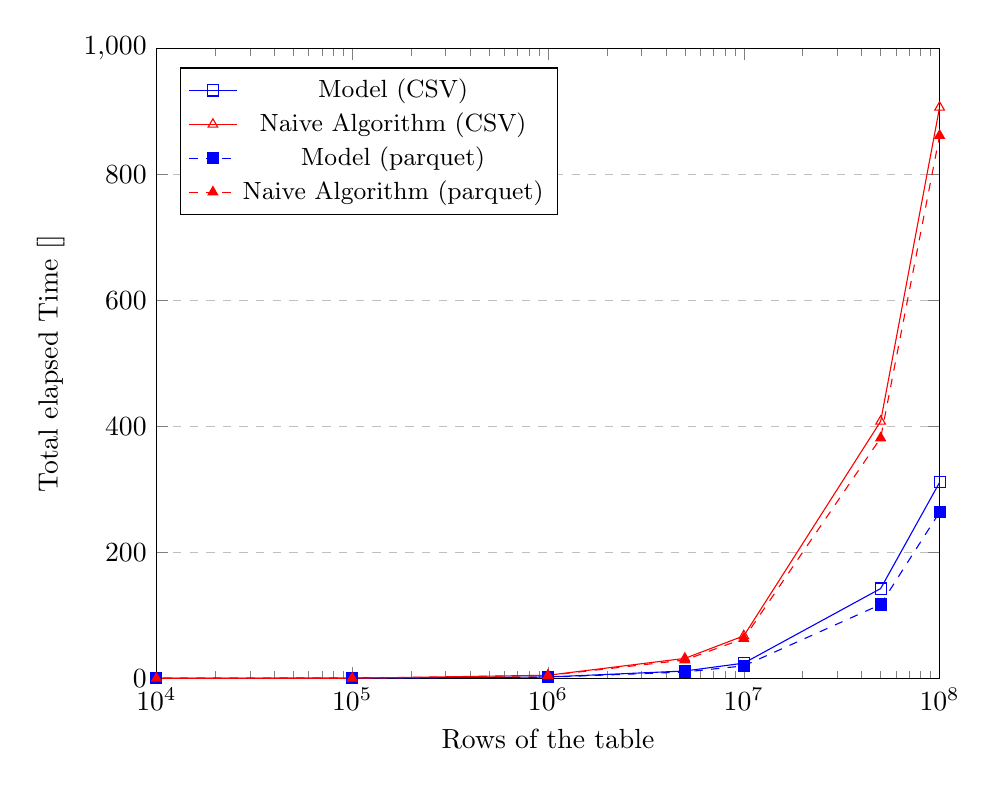
\begin{tikzpicture}
    \begin{axis}[
        % title={},
        xlabel={Rows of the table},
        ylabel={Total elapsed Time [\si{\second}]},
        xmin=10000, xmax=100000000, xmode=log,
        ymin=0, ymax=1000,
        % xtick={0,1000,100000,10000000,100000000},
        % ytick={0,20,40,60,80,100,120},
        legend pos=north west,
        ymajorgrids=true,
        grid style=dashed,
        scale only axis,
        width={\linewidth-62pt},
        height=8cm
      ]

      % csv
      \addplot[
        color=blue,
        mark=square,
      ]
      coordinates {
          (100.0,1.0835406184196472) (1000.0,0.4514627978205681) (10000.0,0.4591604061424732) (100000.0,0.5741918832063675) (1000000.0,2.2600879333913326) (5000000.0,11.771335251629353) (10000000.0,24.25790297240019) (50000000.0,142.64984269440174) (100000000.0,311.1732710637152)
        };

      \addplot[
        color=red,
        mark=triangle,
      ]
      coordinates{
          (100.0,0.0039823874831199) (1000.0,0.0037141181528568) (10000.0,0.0264939442276954) (100000.0,0.3022922314703464) (1000000.0,5.0495885498821735) (5000000.0,31.796920645982027) (10000000.0,67.54112743958831) (50000000.0,408.1332451477647) (100000000.0,906.6464131213723)
        };

      % parquet
      \addplot[
        color=blue,
        mark=square*,
        dashed,
        mark options={solid}
      ]
      coordinates {
          (100.0,0.4577647559344768) (1000.0,0.4482727721333504) (10000.0,0.4571339413523674) (100000.0,0.5343325138092041) (1000000.0,1.90179156512022) (5000000.0,10.232811015099289) (10000000.0,19.938058882951736) (50000000.0,117.29449190944432) (100000000.0,263.89783180877566)
        };

      \addplot[
        color=red,
        mark=triangle*,
        dashed,
        mark options={solid}
      ]
      coordinates{
          (100.0,0.0062335357069969) (1000.0,0.0053194314241409) (10000.0,0.0245211236178874) (100000.0,0.2559473849833011) (1000000.0,4.6651470102369785) (5000000.0,29.216464921832085) (10000000.0,63.27469082176685) (50000000.0,381.673400811851) (100000000.0,861.8326124921441)
        };

      %       % parquet small_table
      %       \addplot[
      %         color=blue,
      %         mark=square,
      %       ]
      %       coordinates {
      % (100.0,0.4629099182784557) (1000.0,0.4608258455991745) (10000.0,0.4631855227053165) (100000.0,1.5644594952464104) (1000000.0,1.8686350099742413) (5000000.0,9.371084868907928) (10000000.0,19.90878576785326) (50000000.0,117.83388417959212) (100000000.0,261.4674338325858) 
      % };

      %       \addplot[
      %         color=red,
      %         mark=triangle,
      %       ]
      %       coordinates{
      % (100.0,0.0039786621928215) (1000.0,0.0044715628027915) (10000.0,0.024229060858488) (100000.0,0.2556539326906204) (1000000.0,4.715674605220556) (5000000.0,29.195809934288263) (10000000.0,63.66628506034613) (50000000.0,381.9564390294254) (100000000.0,861.1740412451327) 
      % };

      \legend{\small Model (CSV), \small Naive Algorithm (CSV), \small Model (parquet), \small Naive Algorithm (parquet)}

    \end{axis}
  \end{tikzpicture}
\end{figure}


\begin{table}[htb]
    \centering
    \begin{tabular}{@{}cccccccccc@{}}
        \toprule
        Rows & Columns & ML: Loading & ML: Compute Time & ML: Loading & ML: Validation Time & ML: Total & Naive: Loading & Naive: Compute Time & Naive: Total \\
        \midrule
        100 & 10 & 0.0285744629800319 & 0.8976177088916302 & 0.0285744629800319 & 0.0001732595264911 & 0.9266809113323689 & 0.0056959092617034 & 0.0005999244749546 & 0.0062979273498058 \\
        1000 & 10 & 0.0037542171776294 & 0.896019458770752 & 0.0037542171776294 & 0.0005894340574741 & 0.9007118158042431 & 0.004017174243927 & 0.0018832795321941 & 0.0059013701975345 \\
        10000 & 10 & 0.0048192664980888 & 0.8991793990135193 & 0.0048192664980888 & 0.0065015368163585 & 0.9108798913657664 & 0.0046558678150177 & 0.0211180038750171 & 0.0257748775184154 \\
        100000 & 10 & 0.0099222585558891 & 0.8982100486755371 & 0.0099222585558891 & 0.0752956457436084 & 0.9840420484542848 & 0.0103398039937019 & 0.2524391710758209 & 0.2627815082669258 \\
        1000000 & 10 & 0.0416129752993583 & 0.9001426883041859 & 0.0416129752993583 & 1.3781779035925863 & 2.3235838785767555 & 0.0510268174111843 & 4.583511143922806 & 4.634541988372803 \\
        10000000 & 10 & 0.469936016947031 & 0.8975801505148411 & 0.469936016947031 & 18.938110906630754 & 20.34980307891965 & 0.4573014304041862 & 63.226555079221725 & 63.683860279619694 \\
        100000000 & 10 & 4.383950512856245 & 0.8998980075120926 & 4.383950512856245 & 257.8179794289172 & 263.50471740216017 & 4.619945663958788 & 861.2739692255855 & 865.8939181752503 \\
        5000000 & 10 & 0.1933269537985324 & 0.9009914770722388 & 0.1933269537985324 & 8.875612087547779 & 10.017441920936108 & 0.1973737850785255 & 28.946411967277527 & 29.143789563328028 \\
        50000000 & 10 & 2.2288895584642887 & 0.9002703092992306 & 2.2288895584642887 & 114.80859450995922 & 118.13907385617496 & 2.192208658903837 & 382.6391819119453 & 384.8313937820494 \\
        \bottomrule
    \end{tabular}
\end{table}
\begin{table}[htb]
    \centering
    \begin{tabular}{@{}cccccccccc@{}}
        \toprule
        Rows & Columns & ML: Loading & ML: Compute Time & ML: Loading & ML: Validation Time & ML: Total & Naive: Loading & Naive: Compute Time & Naive: Total \\
        \midrule
        100 & 10 & 0.0071620605885982 & 1.9453033320605757 & 0.0071620605885982 & 0.0001881271600723 & 1.9559939168393607 & 0.0032919943332672 & 0.0004279762506484 & 0.0037214271724224 \\
        1000 & 10 & 0.0016687996685504 & 1.903506875038147 & 0.0016687996685504 & 0.0006284154951572 & 1.9090951569378376 & 0.0030563995242118 & 0.001796655356884 & 0.0048539713025093 \\
        10000 & 10 & 0.0028518959879875 & 1.9060719460248947 & 0.0028518959879875 & 0.0069547779858112 & 1.9196481332182884 & 0.0043456405401229 & 0.0209928341209888 & 0.0253395251929759 \\
        100000 & 10 & 0.0077248290181159 & 1.9095068275928495 & 0.0077248290181159 & 0.0743687413632869 & 1.9981749355793 & 0.0100578851997852 & 0.2493308521807193 & 0.2593907974660396 \\
        1000000 & 10 & 0.0311676077544689 & 1.908227637410164 & 0.0311676077544689 & 1.3814233131706717 & 3.349048137664795 & 0.0403711609542369 & 4.720485333353281 & 4.760860446840525 \\
        10000000 & 10 & 0.2405276335775852 & 1.911706104874611 & 0.2405276335775852 & 18.850886669009924 & 21.267441116273403 & 0.4768300876021385 & 62.99408712610602 & 63.47092107310891 \\
        100000000 & 10 & 1.6023986004292965 & 1.9012825675308704 & 1.6023986004292965 & 253.95857581868768 & 259.82260693982244 & 4.500701207667589 & 858.0557726882398 & 862.5564770698547 \\
        5000000 & 10 & 0.1172337085008621 & 1.8928483836352823 & 0.1172337085008621 & 8.731336403638124 & 10.85207498818636 & 0.1852367520332336 & 28.96718416363001 & 29.15242387726903 \\
        50000000 & 10 & 1.172201544046402 & 1.887633480131626 & 1.172201544046402 & 114.44143295660616 & 118.8367937207222 & 2.319131284952164 & 379.5390679575503 & 381.8582023233175 \\
        \bottomrule
    \end{tabular}
\end{table}


% \subsection{Comparing models with different input sizes}\label{subsec:efficiency-comparing_models} % TODO: Writing
% Short description of what \enquote{different input sizes} means (long explanation in earlier section).

% Compare times for \SI{70}{\percent}.

% Conclusion: No large difference, the difference may correlate with the larger file size of the model itself.


\subsection{Changing the ratio of unique columns}\label{subsec:efficiency-changing_uniques}
The last variable that has an impact on the runtime of the model is the percentage of unique columns in the table. Since every positive prediction by the model has to be verified using the naive algorithm, the total runtime increases the more unique columns the model detects. The number of unique columns predicted by the model correlates roughly with the number of actual unique columns in the table. % TODO: ref to section under correctness test?

In this experiment, a model with an input size of \num{10} rows is used on \num{4} tables, which are saved as parquet files. The difference between these tables is the percentage of unique columns, which range from \SI{60}{\percent} to \SI{90}{\percent}. Each table has \num{100000000} rows and \num{10} columns.

Table~\ref{table:efficiency-changing_uniques-table} shows that nearly every step of the process takes the same amount of time, just the validation step is proportional to the number of unique columns.

In the GitTables dataset, which is used in the correctness test, the ratio of unique columns is \SI{10}{\percent}. The positive guesses of the model are quite a bit higher since its priority is to avoid false negatives, not false positives. Still, the share of positive guesses during tests on the GitTables dataset is around \SI{30}{\percent}, which is low enough to be a clear improvement over the naive algorithm given large enough tables. %! TODO: percentage of positive guesses

\begin{table}[ht]
    \caption[Efficiency experiment on tables with varying numbers of unique columns]{The result of the efficiency experiment where each table has a size of \num{100000000} rows and \num{10} columns and is read from a parquet file. The only thing that is changing is the number of unique columns.}
    % \small
    \makebox[\linewidth][r]{%
    \begin{tabular}{@{}SSSSSSSS@{}}
        \toprule
        {\shortstack{Unique\\Columns}} & {\shortstack{Model:\\Loading}} & {\shortstack{Model:\\Computing}} & {\shortstack{Model:\\Validation}} & {\shortstack{Model:\\Total}} & {\shortstack{Naive:\\Loading}} & {\shortstack{Naive:\\Computing}} & {\shortstack{Naive:\\Total}} \\
        \midrule
        4 & 4.48926031216979 & 1.3078778870403769 & 344.74235140904784 & 351.12746534124017 & 4.492683906108141 & 861.110518924892 & 865.6032059267163 \\
        3 & 4.47317860648036 & 1.5488394163548946 & 257.4711396209896 & 263.89783180877566 & 4.395280238240957 & 857.4373284652829 & 861.8326124921441 \\
        2 & 4.445464082062244 & 1.1798789985477924 & 171.9837566949427 & 177.8809516504407 & 4.387704025954008 & 862.4403069019318 & 866.8280142992735 \\
        1 & 4.5677355751395226 & 0.4685130454599857 & 87.07020292803645 & 92.24436162412168 & 4.497119572013617 & 856.5085486248136 & 861.0056716166437 \\
        \bottomrule
    \end{tabular}\label{table:efficiency-changing_uniques-table}
    }
\end{table}


\subsection{Summary}\label{subsec:efficiency-summary}
The experiments in this section show that the proposed method of finding primary key candidates is suitable for some cases. If the tables which will be examined contain mostly viewer than \num{1000000} rows or the ratio of unique columns is high, the model is probably slower than the naive algorithm. On very large tables with \num{100000000} or more rows however the model can significantly improve the overall runtime. % maybe something about i/o?

Section~\ref{subsec:efficiency-changing_uniques} additionally demonstrates that it is important for a high efficiency to decrease the number of false positive guesses by the model as much as possible.
